\section{Introduction}

In the previous chapter we

A high level overview of the integration of OmniTune and SkelCL is
shown in Figure~\ref{fig:omnitune-system-flow}.

\begin{figure}
\centering
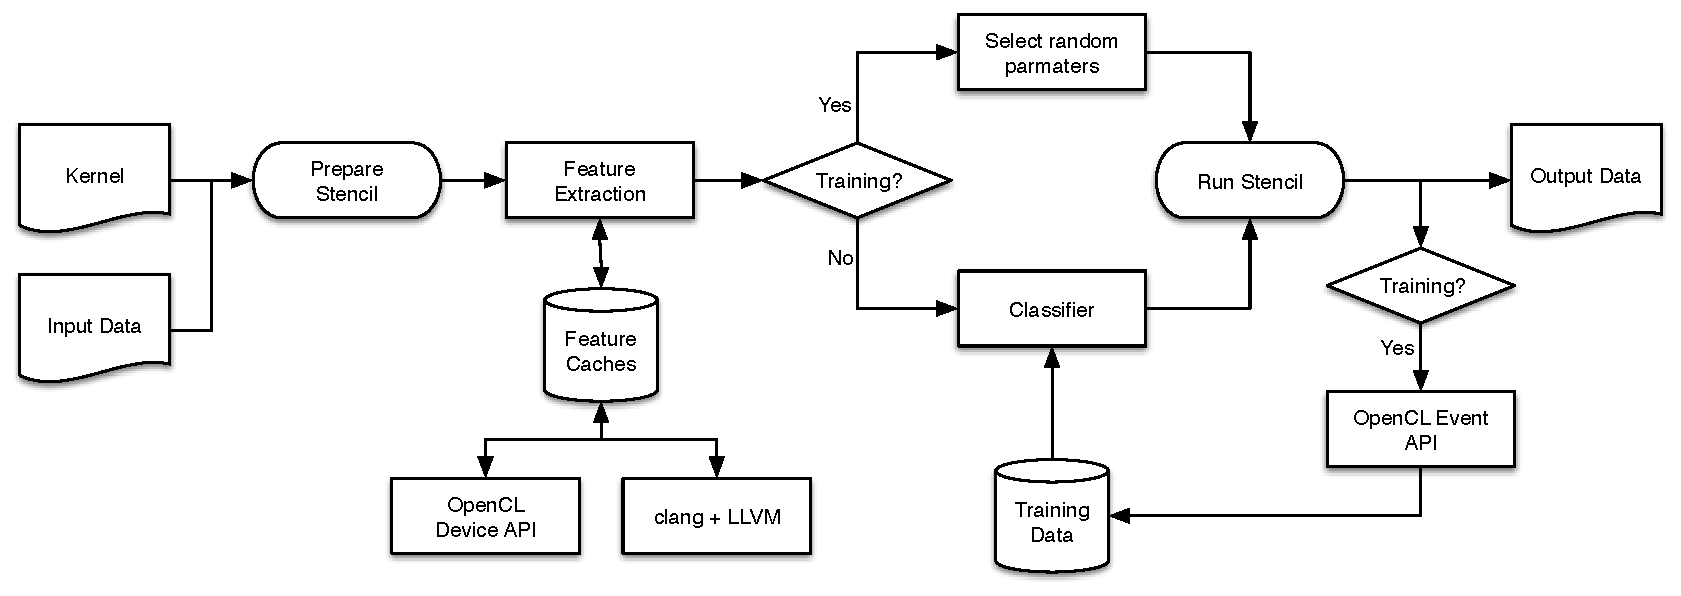
\includegraphics[width=\textwidth]{img/omnitune-system-flow.pdf}
\caption{%
  Integration of OmniTune into SkelCL stencil execution.%
}
\label{fig:omnitune-system-flow}
\end{figure}

\section{Feature Extraction}

As demonstrated in Chapter~\ref{chap:methodology}, the performance of
a workgroup size depends on properties of the architecture, device,
and dataset. The success of a machine learning system depends on the
ability to translate these properties into explanatory variables ---
\emph{features}. For each scenario, a vector of 102 features is
extracted to capture properties of the architecture, device, and
dataset.


\subsubsection{Architectural features}

OmniTune use the OpenCL \texttt{clGetDeviceInfo()} API to query a
number of properties about the target execution device. Examples
include the size of local memory, maximum work group size, number of
compute units, etc.


\subsubsection{Kernel features}

To extract features of the kernel, the user code for the stencil is
passed to the OmniTune server, which compiles the OpenCL kernel to
LLVM IR bitcode. The \texttt{opt} \texttt{InstCount} statistics pass
is used to obtain instruction counts for each type present in the
kernel, and the total number of instructions. The instruction counts
for each type are divided by the total number of instructions to
produce a \emph{ratio} of instruction for that type. Examples include
total static instruction count, ratio of instructions per type, ratio
of basic blocks per instruction, etc.

\TODO{Write an experiment for which static instruction counts fall
  down. For example, two programs with similar instruction counts, one
  with a huge loop, the other with straight line code.}


\subsubsection{Dataset features}

Dataset features are extracted from the SkelCL container type. The
extracted features are the input and output data types, and the 2D
grid size.

See Table~\ref{tab:features} for a full list of features and
types.

\subsubsection{Cost of Feature Extraction}

\TODO{Report feature extraction cost. Note that feature vectors are
  cached so this cost is a one-off, subsequent iterations are just a
  table lookup.}

\begin{table}
\begin{multicols}{2}
\scriptsize
\centering
\rowcolors{2}{white}{gray!25}
\begin{multicols}{2}
\scriptsize
\centering
\rowcolors{2}{white}{gray!25}
\begin{multicols}{2}
\scriptsize
\centering
\rowcolors{2}{white}{gray!25}
\input{gen/tab/features.1}
\vfill
\columnbreak
\rowcolors{2}{white}{gray!25}
\input{gen/tab/features.2}
\end{multicols}

\vfill
\columnbreak
\rowcolors{2}{white}{gray!25}
\begin{multicols}{2}
\scriptsize
\centering
\rowcolors{2}{white}{gray!25}
\input{gen/tab/features.1}
\vfill
\columnbreak
\rowcolors{2}{white}{gray!25}
\input{gen/tab/features.2}
\end{multicols}

\end{multicols}

\vfill
\columnbreak
\rowcolors{2}{white}{gray!25}
\begin{multicols}{2}
\scriptsize
\centering
\rowcolors{2}{white}{gray!25}
\begin{multicols}{2}
\scriptsize
\centering
\rowcolors{2}{white}{gray!25}
\input{gen/tab/features.1}
\vfill
\columnbreak
\rowcolors{2}{white}{gray!25}
\input{gen/tab/features.2}
\end{multicols}

\vfill
\columnbreak
\rowcolors{2}{white}{gray!25}
\begin{multicols}{2}
\scriptsize
\centering
\rowcolors{2}{white}{gray!25}
\input{gen/tab/features.1}
\vfill
\columnbreak
\rowcolors{2}{white}{gray!25}
\input{gen/tab/features.2}
\end{multicols}

\end{multicols}

\end{multicols}

\caption{Feature names and types, describing the dataset, kernel,
  and device.}
\label{tab:features}
\end{table}


\begin{figure}
\centering
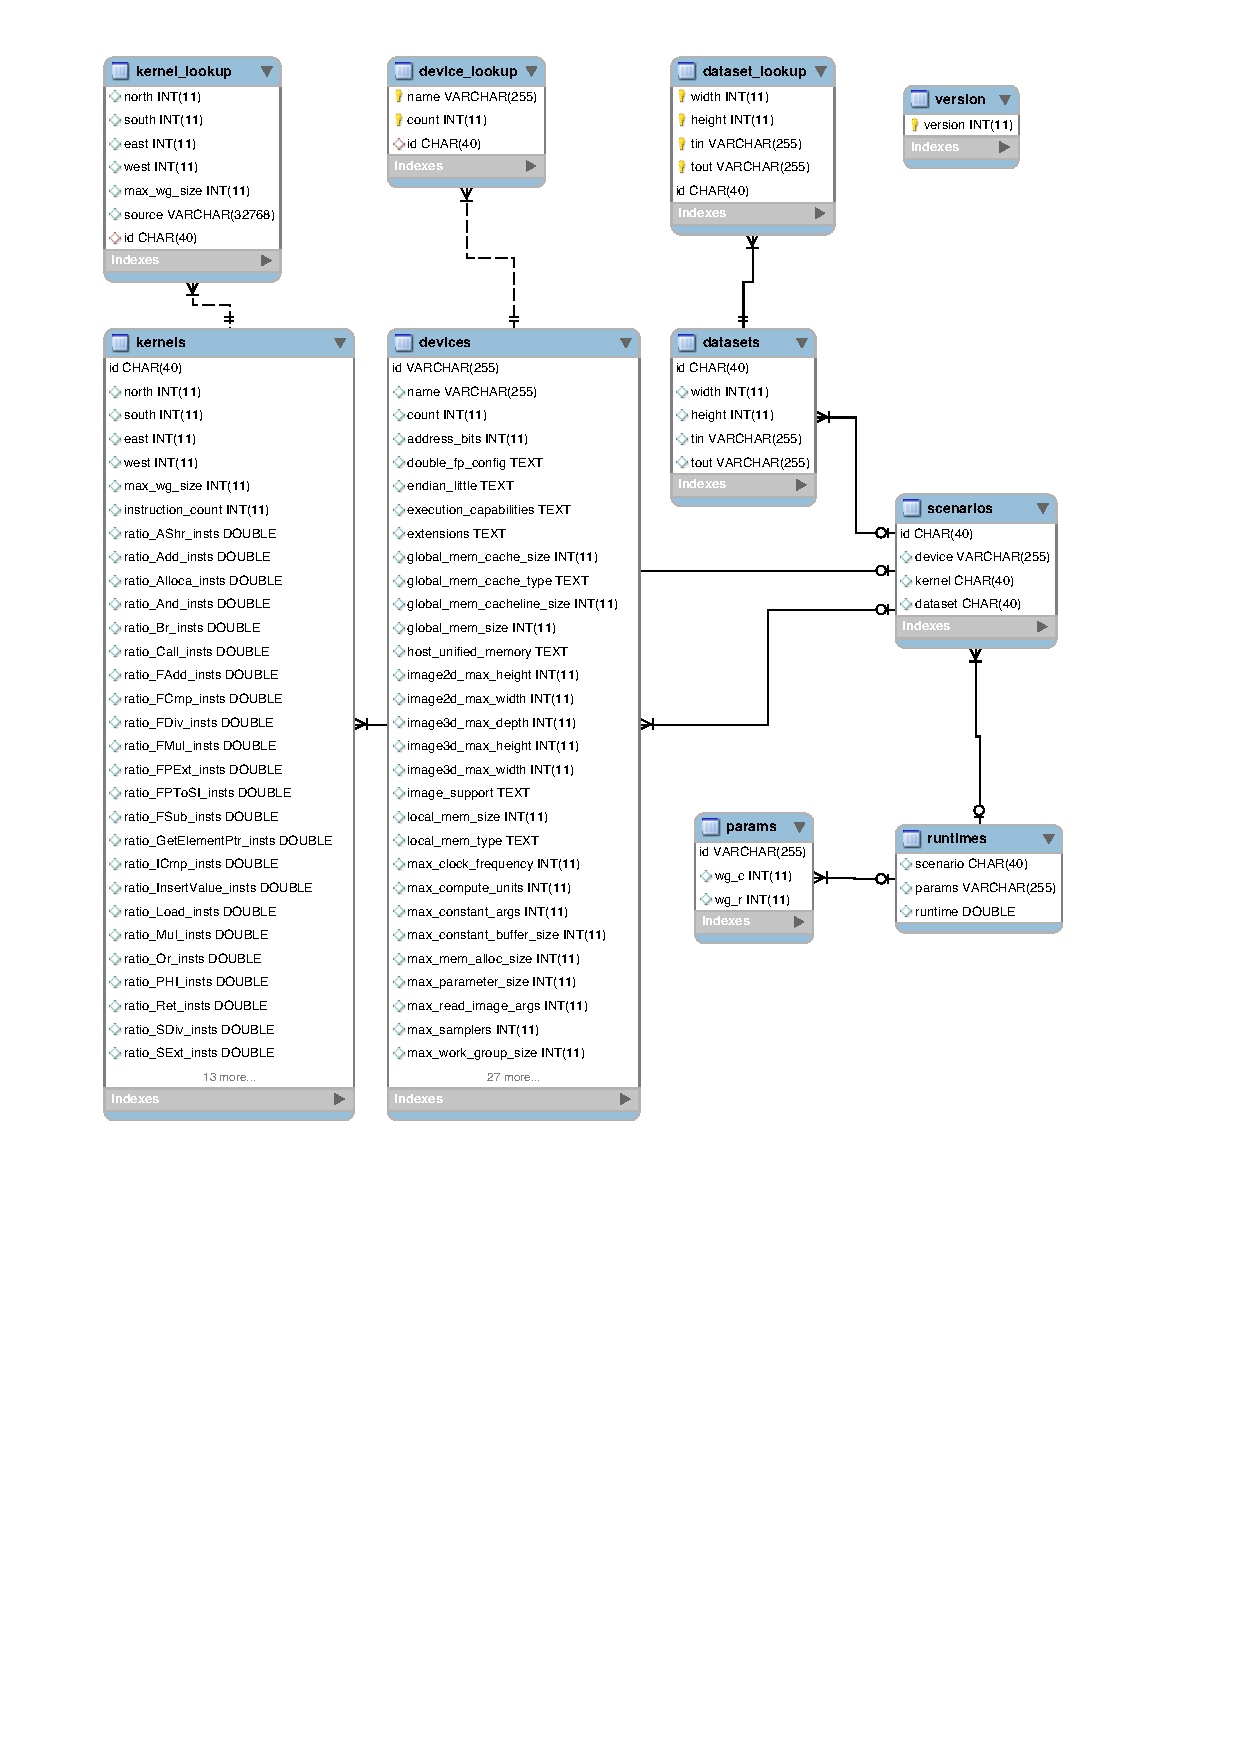
\includegraphics[width=\textwidth]{img/omnitune-data-schema.pdf}
\caption{%
  OmniTune SkelCL schema.%
}
\label{fig:omnitune-system-flow}
\end{figure}


\section{Training}

One challenge of performing empirical performance evaluations is
gathering enough applications to ensure meaningful
comparisons. Synthetic benchmarks are a popular method for
circumventing this issue, by comparing the performance of artificial
workloads. The automatic generation of such benchmarks has clear
benefits for reducing evaluation costs; however, creating meaningful
benchmark programs is a difficult problem if we are to avoid the
problems of redundant computation and produce provable halting
benchmarks (\FIXME{Citations needed, although there will need to be a
  more extensive review of this in the related work chapter}).

In practise, stencil codes exhibit many common traits: they have a
tightly constrained interface, predictable memory access patterns, and
well defined input and output data types. This can be used to create a
confined space of possible stencil codes by enforcing upper and lower
bounds on properties of the codes which can not normally be guaranteed
for general-purpose programs, e.g. the number of floating point
operations. By doing so, it is possible to create a system to
programatically generate synthetic stencil workloads which can
\TODO{\ldots}.

One motivation for the use of synthetic benchmarks is that for the
purposes of autotuning, generating a large set of synthetic benchmarks
can address the ``small $n$, large $P$'' problem, which describes the
difficulty of statistical inference in spaces for which the set of
possible hypotheses $P$ is significantly larger than the number of
observations $n$\CitationNeeded{}. Creating parameterised, synthetic
benchmarks, it is possible to explore a much larger set of the space
of possible stencil codes than if relying solely on reference
applications, for example, to evaluate the performance impact of
highly irregular stencil shapes.

\FIXME{The synthetic benchmarks I've used aren't actually
  \emph{procedurally} generated. I'll either need to implement a
  stencil generator, or failing that, describe my method for creating
  the synthetic benchmarks and move the discussion of procedurally
  generated stencils into the future work section.}

The synthetic benchmarks used in this thesis are parameterised by
stencil shape (one parameter for each of the four directions), input
and output data types (either integers, or single or double precision
floating points), and \emph{complexity} --- a simple metric for
indicating the desired number of memory accesses and instructions per
stencil.


\section{Predicting Workgroup Size}

The optimisation space presented by selection of workgroup size is
large, complex, and non-linear. In this section I apply the techniques
of machine learning and statistical inference to build a system which
is capable of predicting workgroup sizes for unseen programs, based on
previously collected performance data.


\subsection{Predicting Optimal Workgroup Sizes}

The first approach to selecting workgroup sizes is to convert the set
of oracle workgroup sizes into a hypothesis space and then use a
classifier to predict the oracle workgroup size for a given set of
features. To evaluate this approach, a subset of scenarios
$S_{training} \subset S$ are labelled with their oracle workgroup
size. The classifier is trained on this labelled training data, and
tested using a set of unseen scenarios
$S_{testing} = S - S_{training}$. The performance of each predicted
oracle workgroup size is compared against the true oracles for that
set.


\subsubsection{Satisfying Constraints}

The set of workgroup sizes which a classifier may predict is defined
by the oracle workgroup sizes of the training data:

\begin{equation}
W_{training} = \{ \Omega(s) | s \in S_{training} \}
\end{equation}

This does not guarantee that the set of workgroup sizes which may be
predicted is within the set of legal workgroup sizes for each tested
scenario:

\begin{equation}
W_{training} \nsubseteq \cup \{ W_{legal}(s) | s \in S_{testing} \}
\end{equation}

\TODO{2 solutions: satisfy constraint at classification time
  (i.e. error handlers), or at training time (i.e. one classifier per
  max-wg-size)\ldots}

As a result, it is possible that a classifier will predict a workgroup
size that is invalid for a given scenario, $w \not\in W_{legal}(s)$.
For these cases, I evaluate the effective of three fallback strategies
to select a legal workgroup size:

\begin{enumerate}
\item \emph{Baseline} --- select the workgroup size which is known to
  be safe and provides the highest average case performance on
  training data.
\item \emph{Random} --- select a random workgroup size which is known
  to be legal $w \in W_{legal}(s)$.
\item \emph{Reshape} --- scale the predicted workgroup size
  proportionally so that it fits within the space of legal workgroup
  sizes, $w < W_{max}(s)$. This attempts to preserve ``shape'' of the
  predicted workgroup size.
\end{enumerate}

See Algorithm~\ref{alg:autotune-classification} for definitions. The
evaluation compares the average performance achieved using each
fallback strategy, along with the percentage of cases for which these
fallback strategies were required.


\begin{algorithm}
\begin{algorithmic}[1]
\Require kernel features $k$, hardware features $h$, dataset features
$d$.
\Ensure workgroup size $w$

\Procedure{Default}{w, a, k, d}
\Comment Use the best safe param.
\State $w \leftarrow \text{classify}(a, k, d)$
\If{$w \in W_{legal}(s)$}
    \State \textbf{return} $w$
\Else
  \State \textbf{return} $\underset{w \in W_{safe}}{\argmax}
\left(
  \prod_{s \in S_{training}} p(s, w)
\right)^{1/|S_{training}|}$
\EndIf
\EndProcedure
\item[]

\Procedure{Random}{w, a, k, d}
\Comment Use a random param from $W_{legal}$.
\State $w \leftarrow \text{classify}(a, k, d)$
\If{$w \in W_{legal}(s)$}
    \State \textbf{return} $w$
\Else
  \State \textbf{return} random choice $w \in W_{legal}$
\EndIf
\EndProcedure
\item[]

\Procedure{Reshape}{w, a, k, d}
\Comment Coerce params to be legal.
\State $w \leftarrow \text{classify}(a, k, d)$
\If{$w \in W_{legal}(s)$}
    \State \textbf{return} $w$
\Else
  \State $d_{min} \leftarrow \infty$
  \State $w_{closest} \leftarrow \text{null}$
  \For{$c \in W_{legal}$}
    \State $d \leftarrow \sqrt{\left(c_r - w_r\right)^2 + \left(c_c - w_c\right)^2}$
    \If{$d < d_{min}$}
      \State $d_{min} \leftarrow d$
      \State $w_{closest} \leftarrow c$
    \EndIf
  \EndFor
  \State \textbf{return} $w_{closest}$
\EndIf
\EndProcedure
\end{algorithmic}

\caption{Select optimal workgroup size using classification}
\label{alg:autotune-classification}
\end{algorithm}


\begin{algorithm}
\begin{algorithmic}[1]
\Require kernel features $k$, hardware features $h$, dataset features
$d$.
\Ensure workgroup size $w$

\State $C \leftarrow \phi$
\Comment Set of classifiers.
\State $W_{training} \leftarrow \{ W_{legal}(s) | s \in S_{training}
\}$

\For{$W_c \in W_{training}$}
  \State $S_c \leftarrow \{ s | s \in S_{training}, W_{legal}(s) = W_c
  \}$
  \Comment Training data with same legal params.
  \State $c \leftarrow \text{\sc{TrainClassifier}}(S_c)$
  \Comment Build a classifier with training data.
  \State $C \leftarrow C \cup \{ c \}$
\EndFor

\State $c \leftarrow C_{W_{legal}(s)}$

\State \textbf{return} $c(a, k, d)$
\end{algorithmic}

\caption{Select optimal workgroup size using multiple classifiers}
\label{alg:autotune-classification2}
\end{algorithm}


\TODO{Implement and evaluate classification using one classifier for
  each unique $w \in \cup \{ W_{max}(s) | s \in S_{training} \}$. This
  would be an alternative method of overcoming the invalid prediction
  problem.}

\subsection{Predicting Stencil Code Runtime}

\TODO{The first approach requires very expensive training and isn't
  amenable to online tuning\ldots} A second approach to selecting the
workgroup size is to attempt to directly predict the runtime of a
given workload. Given a regressor $f(a,k,d,w)$ which predicts the
runtime of a program given a set of architecture, kernel, and dataset
features $a,k,d$, and workgroup size $w$, the predicted optimal
workgroup size is the $w$ value which minimises the output of the
regressor:

\begin{equation}
  \underset{w \in W_{legal}(s)}{\argmin} f(a,k,d,w)
\end{equation}

By predicting the runtimes of only the workgroup sizes from within
$W_{legal}(s)$, we overcome the issue of predicting invalid workgroup
sizes. Training a regressor to predict runtimes requires a set of
training data which contains workgroup sizes as an additional feature,
and the measured mean runtime as the label.

% \begin{algorithm}
% \begin{algorithmic}[1]
\Require kernel features $k$, hardware features $h$, dataset features
$d$.
\Ensure predicted oracle workgroup size $\bar{\Omega}(s)$
\State $C \leftarrow \{c_1, c_2, \ldots, c_n \}$
\Comment Set of all workgroup sizes $\le k.\text{max\_wgsize}$
\State \textbf{return} $\underset{c \in C}{\argmin} f(k,h,d,c)$
\end{algorithmic}

% \caption{Selecting workgroup size using runtime regression}
% \label{alg:autotune-runtime-regression}
% \end{algorithm}

\subsection{Predicting Relative Performance}

Accurately predicting the runtime of an arbitrary program is a
difficult problem due to the impacts of flow control. It may be
effective to instead predict the \emph{relative} performance of two
different workgroup sizes for the same program. To do this, we select
a baseline workgroup size $w_b \in W_{safe}$, and train a regressor
$g(a,k,d,w)$ with training data labelled with the relative performance
over the baseline $r(w, w_b)$. Predicting the optimal workgroup
requires maximising the output of the regressor:

\begin{equation}
  \underset{w \in W_{legal}(s)}{\argmax} g(a,k,d,w)
\end{equation}

% \begin{algorithm}
% \begin{algorithmic}[1]
\Require kernel features $k$, hardware features $h$, dataset features
$d$.
\Ensure workgroup size $w$
\State $C \leftarrow \{c_1, c_2, \ldots, c_n \}$
\Comment Set of all workgroup sizes $\le k.\text{max\_wgsize}$
\State \textbf{return} $\underset{c \in C}{\argmax} f(k,h,d,c)$
\end{algorithmic}

% \caption{Selecting workgroup size using speedup regression}
% \label{alg:autotune-speedup-regression}
% \end{algorithm}


\subsection{Meta-tuning: a Hybrid Approach}

\TODO{Implement and test. See Algorithm~\ref{alg:autotune-hybrid}.}

\begin{algorithm}
\begin{algorithmic}[1]
\Require kernel features $k$, hardware features $h$, dataset features $d$.
\Ensure workgroup size $w$

\State $r \leftarrow \underset{w \in W_{legal}(s)}{\min} f(k,h,d,w)$
\Comment Predict minimum runtime.
\State $w \leftarrow \underset{w \in W_{legal}(s)}{\argmin} f(k,h,d,w)$
\Comment Workgroup size for $r$.
\State $t_r \leftarrow$ measure runtime of program with $w$
\If{$t_r \approx r$}
  \State \textbf{return} $w$
\Comment Predicted runtime is accurate.
\Else
   \State $W \leftarrow W_{legal}(s)$
   \State converged $\leftarrow$ false
   \State $w_b \leftarrow$ baseline value
   \State $t_b \leftarrow$ measure runtime of runtime of program with $w_b$
   \While{not converged}
     \State $s \leftarrow \underset{w \in W}{\max} g(k,h,d,w)$
     \Comment Predict best speedup.
     \State $w \leftarrow \underset{w \in W}{\argmax} g(k,h,d,w)$
     \Comment Workgroup size for $s$.
     \State $t \leftarrow$ measure runtime of program with $s$
     \If{$t_b / t \approx s$}
       \State converged = true
       \Comment Predicted speedup is accurate.
     \Else
       \State $W = W - \{w\}$
     \EndIf
   \EndWhile
   \State \textbf{return} $w$
\EndIf
\end{algorithmic}

\caption{Selecting workgroup size using a hybrid approach}
\label{alg:autotune-hybrid}
\end{algorithm}


\section{Summary}
